\section{Dziedzina problemu}

\begin{wrapfigure}{R}{3in}
%%%%%%%%%%%%%%%%%%%%%%%%%%%%%%%%%%%%%%%%%%%%%%%%%%%%%%%%%%%%%%%%%%%%%%%%%%%%%%%%%%%%%%%
%%% You will need to add \usepackage{wrapfig} to your preamble to use textwrapping %%%
%%%%%%%%%%%%%%%%%%%%%%%%%%%%%%%%%%%%%%%%%%%%%%%%%%%%%%%%%%%%%%%%%%%%%%%%%%%%%%%%%%%%%%%
 \centering
 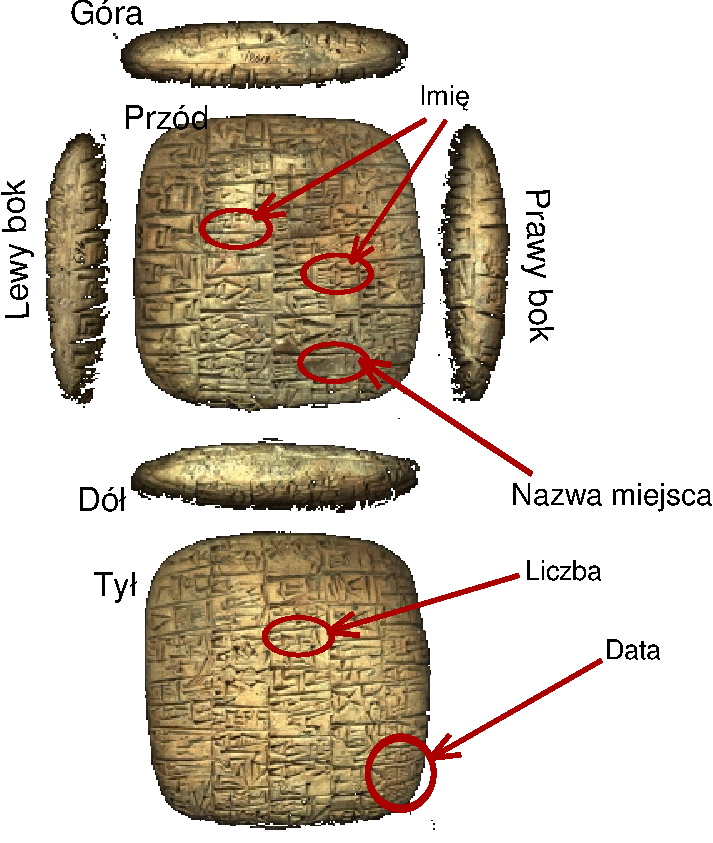
\includegraphics[width=150px]{../diagramy/tabliczka.pdf}
 % tabliczka.pdf: 342x405 pixel, 72dpi, 12.06x14.29 cm, bb=0 0 342 405
 \caption{\label{fig:tabliczka}Gliniana tabliczka -- struktura}
\end{wrapfigure}


% \begin{figure}[h]
%  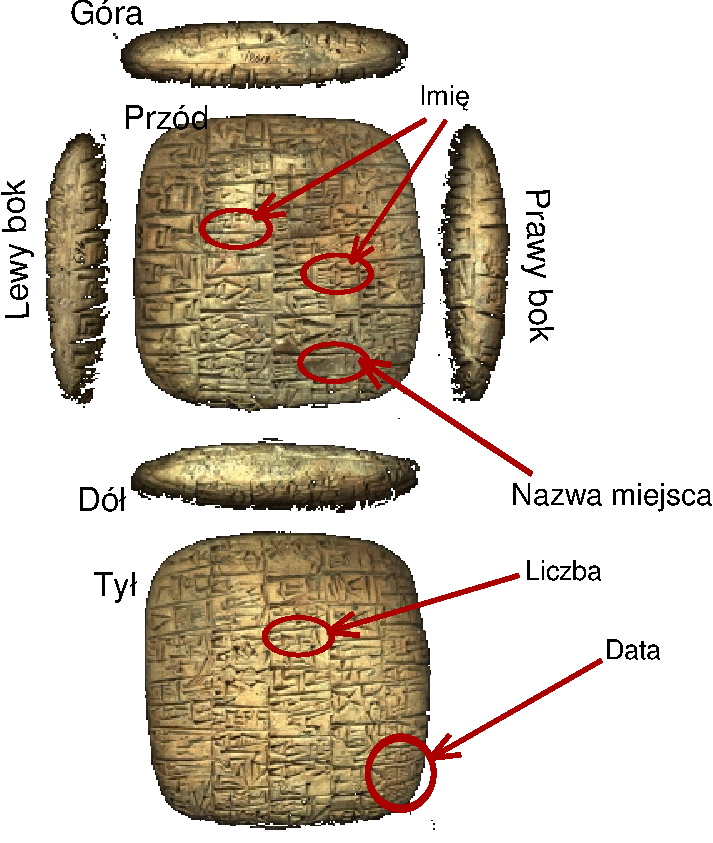
\includegraphics[width=150px]{../diagramy/tabliczka.pdf}
%  % tabliczka.pdf: 342x405 pixel, 72dpi, 12.06x14.29 cm, bb=0 0 342 405
%  \caption{Gliniana tabliczka - struktura}
% \end{figure}

Podstawowym elementem rozpatrywanej przez nas dziedziny jest \emph{tabliczka sumeryjska}. 
Pojęcie to odnosi się zarówno do fizycznej \emph{tabliczki glinianej} jak i do jej cyfrowej reprezentacji, 
odpowiedniej do przechowywania na komputerze. 

Tabliczki gliniane mają różne kształty i rozmiary. 
Mogą być zapisane z wielu stron (z przodu, z tyłu, od góry, z boku, itp.), a także mogą zawierać pieczęcie, 
na których również znajduje się tekst. Przez kilka tysięcy lat istnienia ulegały też uszkodzeniom uniemożliwiającym 
obecnie ich pełne odczytanie.
Przykładowa gliniana tabliczka zaprezentowana jest na rysunku \ref{fig:tabliczka}.

% akapit o samym piśmie klinowym
Tekst na tabliczkach jest zapisany za pomocą \emph{klinów}. Pismo klinowe jest prawdopodobnie najstarszym pismem na świecie 
(konkurują z nim jedynie hieroglify egipskie)  \cite{kuckenburg}. Początkowo składało się z piktogramów z czasem coraz bardziej upraszczanych.
Służyło pomocą w rozliczeniach i umowach, zapisywano np. ilość i rodzaj obiecanych ludziom zwierząt.

Treść tabliczek to najczęściej dokumenty urzędowe dotyczące czynności administracyjnych i gospodarczych, 
produkcji i dystrybucji rozmaitych artykułów, uroczystości religijno--kulturowych, umów cywilnoprawnych itp. \cite{powalka}
Często można spotkać w niej między innymi imiona osób i bóstw, liczby, jednostki (np. mina -- jednostka wagi), % sprawdziłam
miejsca, daty. Niektóre z tych elementów można przetłumaczyć na współczesny język, na przykład jednostki można przeliczyć na SI, 
datę opisową na datę wg obecnego kalendarza gregoriańskiego. 

Dla ułatwienia pracy sumerolodzy tłumaczą zapis klinowy na tzw. \emph{odczyty}. 
Są one sposobem zapisania tekstu sumeryjskiego za pomocą współczesnych znaków -- liter alfabetu łacińskiego i cyfr arabskich, 
na podstawie prawdopodobnego brzmienia słów w języku sumeryjskim. 
W tłumaczeniu uwzględniony jest także kształt tabliczki i rozmieszczenie poszczególnych fragmentów tekstu 
(zgodnie z rysunkiem \ref{fig:tabliczka}). 
 
Odczyty zawarte w cyfrowym zapisie tabliczki są tylko jednym z wariantów tłumaczenia z klinów. 
Przede wszystkim dlatego, że jeden klin może zostać odczytany na wiele różnych sposobów. 
Ponadto odczytowi może odpowiadać nie tylko jeden klin, ale także ich sekwencja. 
Ponieważ w cyfrowej wersji nie ma klinów, trudno jest zweryfikować ewentualne pomyłki w tłumaczeniach.

W takiej właśnie formie tabliczki elektroniczne są przechowywane w pamięci komputerów. 
Niestety ten zapis może być mylący ze względu na niejednoznaczności występujące przy tłumaczeniu. 

% Pomocne mogłoby by narzędzie, które pozwala wyszukiwać również w alternatywnych tłumaczeniach.
Źródłem dodatkowych problemów są uszkodzenia tabliczek. 
W wielu przypadkach naukowcy mogą domyślić się jak wyglądał brakujący fragment. 
Zawsze natomiast informację o uszkodzeniu oraz domniemaną brakującą treść zapisują w tabliczce cyfrowej.
Ponieważ pewne konwencje opisywania tych informacji zostały przyjęte dosyć późno i nie przez wszystkich sumerologów, 
są one zapisywane na różne sposoby. Również tutaj możliwe są pomyłki i niejednoznaczności.

\begin{figure}[h]
 \centering
 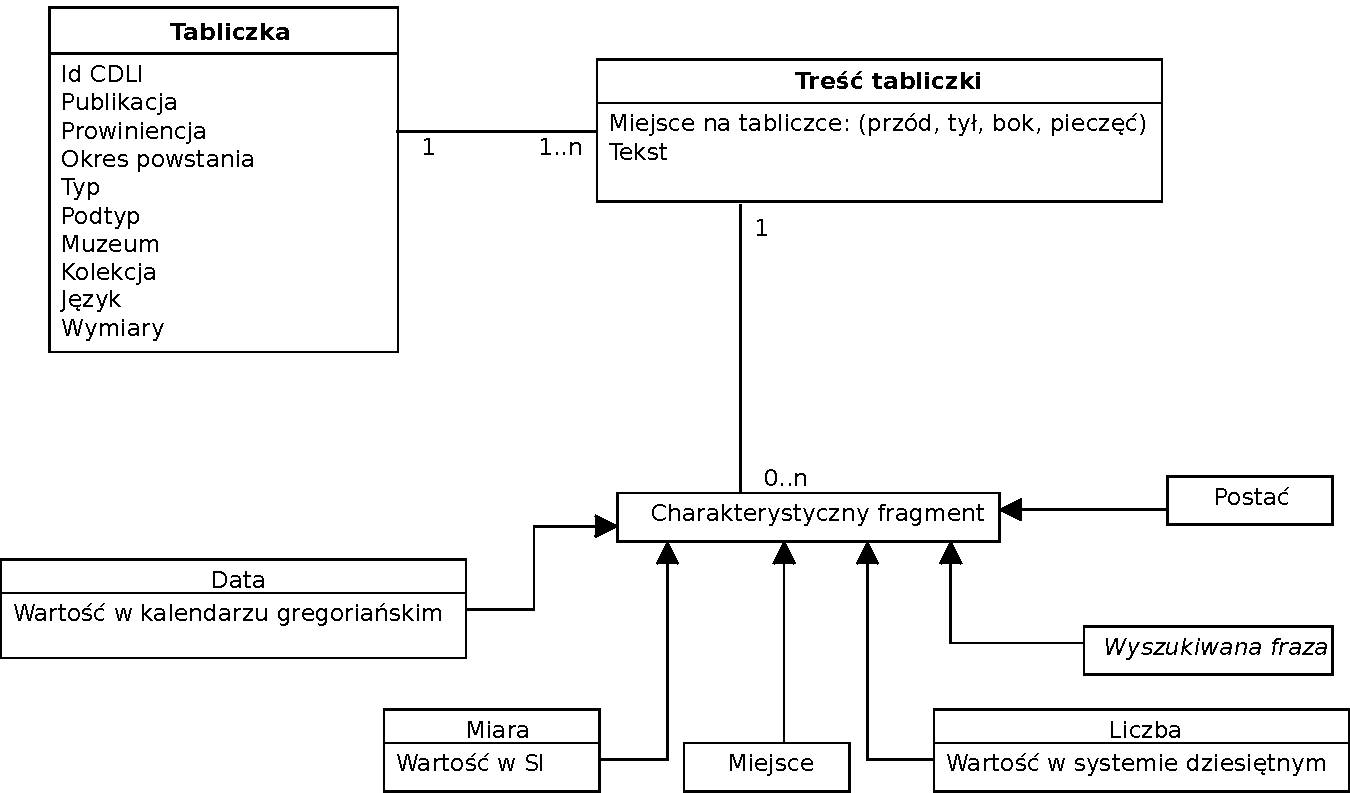
\includegraphics[width=400px]{../diagramy/Model-dziedziny.pdf}
 % Model-dziedziny.png: 650x345 pixel, 72dpi, 22.93x12.17 cm, bb=0 0 650 345
 \caption{\label{fig:cyfrowa_tab}Co powinna zawierać cyfrowa reprezantacja tabliczki}
\end{figure}
Tabliczka cyfrowa, oprócz treści, zawiera także informacje, które nie były zawarte na tabliczce glinianej 
(rysunek \ref{fig:cyfrowa_tab}). 
Są to metadane, takie jak miejsce znalezienia tabliczki, okres, w którym powstała, czy nazwa kolekcji, do której obecnie należy. 
Te informacje są istotne przy przeszukiwaniu, gdyż często pozwalają na określenie o czym jest tabliczka bez dokładnej analizy 
jej treści. 
W praktyce, wśród sumerologów, atrybutem, który w znacznym stopniu pomaga zidentyfikować tabliczkę, jest informacja o jej publikacji.

Nie ma wątpliwości, że cyfrowa postać tabliczek sumeryjskich wraz z podstawowymi możliwościami wyszukiwania znacząco
ułatwia sumerologom ich badania. Brakuje im jednak możliwości znajdowania tabliczek na podstawie
bardziej skomplikowanych i rozbudowanych kryteriów.
Wychodząc naprzeciw tej potrzebie, chcemy stworzyć język, w którym będą oni mogli w łatwy sposób wyrażać, 
jakich tabliczek potrzebują, i który jednocześnie będzie można wykorzystać do przeszukiwania baz danych. 
Język ten powinien przede wszystkim umożliwiać wyszukiwanie na podstawie treści tabliczki (odczytów), 
alternatywnych tłumaczeń (wymaga to przetłumaczenia tabliczki z powrotem na kliny) oraz metadanych.
Dodatkową zaletą byłoby wyszukiwanie po specyficznych fragmentach (tagach), takich jak imiona, jednostki, daty.
W pierwszej wersji języka implementujemy tylko wyszukiwanie po odczytach i metadanych.